\documentclass[10pt,twocolumn,letterpaper]{article}

\usepackage{cvpr}
\usepackage{times}
\usepackage{epsfig}
\usepackage{graphicx}
\usepackage{amsmath}
\usepackage{amssymb}
\usepackage{float}

% Include other packages here, before hyperref.
\setlength{\intextsep}{8pt plus 2pt minus 2pt}

% If you comment hyperref and then uncomment it, you should delete
% egpaper.aux before re-running latex.  (Or just hit 'q' on the first latex
% run, let it finish, and you should be clear).
\usepackage[breaklinks=true,bookmarks=false]{hyperref}

\cvprfinalcopy % *** Uncomment this line for the final submission

\def\cvprPaperID{****} % *** Enter the CVPR Paper ID here
\def\httilde{\mbox{\tt\raisebox{-.5ex}{\symbol{126}}}}

% Pages are numbered in submission mode, and unnumbered in camera-ready
%\ifcvprfinal\pagestyle{empty}\fi
\setcounter{page}{1}
\begin{document}
\vspace{-0.5cm}

%%%%%%%%% TITLE

\title{EE3 Deep Learning Interim Report}
\vspace{-0.5cm}

\author{Alexander Montgomerie-Corcoran\\
{\tt\small CID: 01052454, am9215@ic.ac.uk}
}

\maketitle
\vspace{-0.3cm}
%\thispagestyle{empty}


%%%%%%%%% ABSTRACT
\begin{abstract}

   This work investigates verification, matching and retrieval tasks for the N-HPatches dataset, a noisy version of the HPatches dataset \cite{hpatches_2017_cvpr}.
   A baseline approach is taken by first performing denoising using an auto-encoder architecture, and descriptor learning using a convolutional neural network feature extractor. The baseline method achieves \textbf{0.086 mAP} for matching, \textbf{0.64 mAP} for retrieval and \textbf{0.68 mAP} for verification.
\end{abstract}

%TODO: add i
\vspace{-0.7cm}

%%%%%%%%% BODY TEXT
\section{Introduction}

\vspace{-0.2cm}
\subsection{Dataset}
\vspace{-0.2cm}

The HPatches dataset consists of sequences of patches extracted from various images. For every reference image, there is a set of patch sequences for the same subject with either viewpoint changes or illumination changes. These illumination variations can be characterised as varying brightness across the reference image. Viewpoint changes come from different perspectives of the subject, as well as artificial geometric noise applied to the patches. These non-reference sequences are ranked by the magnitude of their viewpoint and illumination variation, and are either \textit{easy, hard} or \textit{tough}. N-HPatches has an additional random pixel noise applied to each patch, with the intensity of this noise based on the patch's rank.
\vspace{-0.2cm}
\subsection{Tasks}
\vspace{-0.2cm}
The N-HPatches dataset is used for three different problem classes. 
The patch verification task consists of classifying the similarity of individual patches. This is done by calculating a distance metric between two descriptors of the reference and test patch.
Image matching tasks compare a pair of patch sequences of two images to determine if they are from the same image. A similar distance metric is applied to the pair of sequences.
The patch retrieval task finds a patch corresponding to the reference patch within a pool of patches.

\vspace{-0.4cm}
\section{Baseline Approach}
\vspace{-0.2cm}

The baseline method separates the problem into denoising and descriptor learning, and employs popular methods for each.
%The baseline approach takes a uniform approach to each task, and splits up the problem into two sections: patch denoising and patch descriptor.

\vspace{-0.2cm}
\subsection{Patch Denoising}
\vspace{-0.2cm}
The patch denoising network makes use of U-Net \cite{RonnebergerFB15}, a popular image segmentation network with use in denoising tasks aswell \cite{GraisP17}. This network
acts as an autoencoder, extracting a reduced set of features with the encoder path, and decoding. Skip connections are used to propgate any information lost during encoding. 
This network is trained on noisy images evaluated against noiseless images, using MAE loss. 

%Figure \ref{fig:denoise_loss} shows that it is able to converge to reach both low validation and training loss, however looking at example outputs in Figure \ref{fig:denoise_image}, there is obvious variation between the example and denoised image. Specifically, there is significantly more blurriness compared to the clean network. Although the network appears to have trained well, it has not captured the significant discriminative features of each patch, due the averaging of the loss function.

% could also look at this problem in a different domain.  
\vspace{-0.2cm}
\subsection{Patch Descriptor}
\vspace{-0.2cm}
A network is defined to extract discriminant features of each patch. This network is derived from L2-Net, a patch descriptor network which employs deep learning techniques.
The network consisted of convolutional layers which extract shift-invariant features of the patch. A fully connected layer is used to obtain the most significant features. This network is trained with triplet loss. The network learns features such that the L2 distance is maximised between reference and negative features, and minimised between positive and reference features.
% TODO: report timing, all that shit

\vspace{-0.2cm}
\subsection{Evaluation}
\vspace{-0.2cm}
Tables \ref{tab:baseline_match}, \ref{tab:baseline_verification} \& \ref{tab:baseline_retrieval} show the results obtained from the benchmark.
The baseline network achieves low precision compared to the baseline results of HPatches, even given the extra noise\footnote{http://cmp.felk.cvut.cz/~mishkdmy/slides/HardNet2017.pdf}. There is therefore significant improvements that can be made regarding denoising.

\vspace{-0.2cm}
\section{Improved Approach}
\vspace{-0.2cm}

To improve on the existing, this new method addresses two aspects to the problem. Firstly, the network architecture attempts to directly reduce the impact of various noise applied to the images. Secondly, loss functions used in the baseline approach are reviewed in order to find the optimal learning method for the network. 

%To improve on the de-noising network, loss functions such as L1 loss and SISSM will be investigated, as they have proven more appropriate for image reconstruction tasks \cite{something}. 

%TODO: network map

%To improve on the de-noising network, loss functions more appropriate for image-based tasks such as SSIM \cite{ZhaoGFK15}will be investigated. As the denoise network uses an averaging loss, there is inherent blurriness at the output such as in Fig. \ref{fig:denoise_image}. Further improvements can be made by assuming additive noise, reducing the compexity of the networks.

%An initial improvement can be made to the descriptor network by identifying existing networks \cite{Tian_2017_CVPR}\cite{Serra_2015_ICCV}\cite{BalntasJTM16}\cite{BMVC2016_119} with better performance, such as HardNet \cite{MishchukMRM17}.
%It would be interesting to investigate domain transforms on the data, such as 2D FFT \cite{rippel2015spectral}, and how this could improve on discriminative ability of the network. A general goal is to address geometric noise more directly.
%It would interesting to expand on this by transforming the domain of the data, appling kernel methods within the network, in particular, how kernels such as the radial basis function can improve discriminative features of the descriptors.

\subsection{Improved Denoise Network}
In the baseline approach, an autoencoder approach is taken towards the problem of denoising images. The problem with the auto-encoder technique is that the encoding path attempts to learn generative features of the image, impeding the ability to learn more discriminative features for the actual descriptor network. 


Another factor explored with the denoise network was varying the loss function. Loss functions such as \textit{mean absolute error} and  \textit{mean squared error} lead to more blurry images due to the averaging techniques used. This work evaulates two different loss functions: SSIM loss and PSNR loss, given by Equations \ref{eq:ssim} and \ref{eq:psnr} respectively. 

%TODO: write loss functions

These loss functions attempt to address the image noise whilst keeping strong features of the image, as there is less averaging used in these techniques. 

\subsection{Improved Descriptor Network}

To address both geometric noise and illumination variance across patches, two additional components are introduced into the network: a spatial transform layer and a sobel filter. 

The spatial transform network (STN) layer attempts to learn affine transforms which reduce the geometric noise between pairs of patches. From the HPatches paper \cite{hpatches}, it is known that geometric noise introduced into the system is caused by affine transformations applied to the patches. This creates difficulties for traditional CNN networks, as they are able to learn translation-invariant features however struggle to learn affine-transform-invariant features, with only pooling layers addressing this sort of invariance TODO: cite. The STN layer attempts to address this. By learning feautures such as patch orientation and so on, these feautures can be used to create coefficients which are able to align the geometrically-distorted patches to their orignal view.

From Figure \ref{fig:stn_output}, it can be seen that the ...

%It is worth noting that it may seem contradictory to use a CNN to learn affine transforms where previously  

The other type of noise introduced into the network is illumination invariance. The approach taken in this work is to use a sobel filter in order to remove any illumination across the image and only give structural features of the patch. From figure \ref{fig:sobel_filter_output}, it can be seen that only edges within the patch are observed at the output, thus removing features caused by uniform illumination across the patch.

%TODO: evaluate illumination invariance across dataset (get mae)
 
{\small
\bibliographystyle{ieee}
\bibliography{egbib}
}

\begin{figure}[H]
\centering
  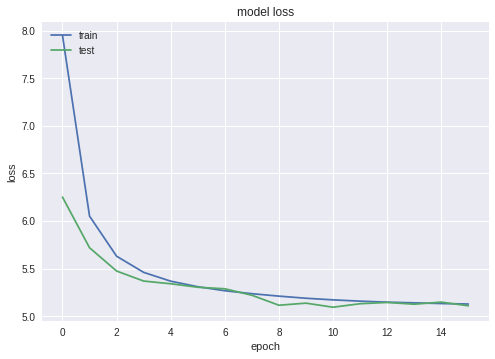
\includegraphics[width=0.65\linewidth]{figures/denoise_train.png}
  \caption{Denoising Network Loss against Epochs.}
  \label{fig:denoise_loss}
\end{figure}


\begin{figure}[H]
\centering
  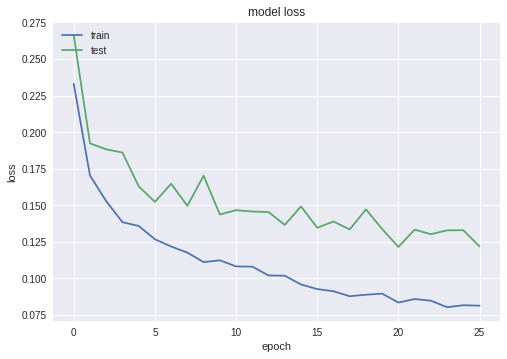
\includegraphics[width=0.65\linewidth]{figures/descriptor_train.png}
  \caption{Descriptor Network Loss against Epochs.}
  \label{fig:descriptor_loss}
\end{figure}

\begin{figure}[H]
\centering
  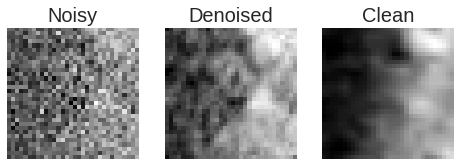
\includegraphics[width=0.65\linewidth]{report/figures/denoise_image.png}
  \caption{Denoising Network Output Example.}
  \label{fig:denoise_image}
\end{figure}


\begin{table}[h]
\centering
\begin{tabular}{| c | c | c | c |}
\hline
Easy     & Hard      & Tough     & mean      \\
\hline
0.176 & 0.061 & 0.021 & 0.086 \\
\hline
\end{tabular}
\caption{Image Matching Task precision results.}
\label{tab:baseline_match}
\end{table}

\begin{table}[h]
\centering
\begin{tabular}{| c | c | c |}
\hline
Noise & Inter    & Intra    \\
\hline
Easy  & 0.806 & 0.721 \\
Hard  & 0.739 & 0.627 \\
Tough & 0.658 & 0.536 \\
\hline
\end{tabular}
\caption{Image Verification Task precision results.}
\label{tab:baseline_verification}
\end{table}

\begin{table}[h]
\centering
\begin{tabular}{| c | c | c | c | c | c | c | c |}
\hline
Noise & 100      & 500      & 1000     & 5000     & 10000     & 15000     & 20000     \\
\hline
Easy  & 0.719 & 0.570 & 0.513 & 0.390 & 0.343 & 0.318 & 0.303 \\
Hard  & 0.648 & 0.451 & 0.376 & 0.232 & 0.185 & 0.162 & 0.149 \\
Tough & 0.557 & 0.33  & 0.254 & 0.127 & 0.093 & 0.078 & 0.07  \\
mean  & 0.641 & 0.45  & 0.381 & 0.25  & 0.207 & 0.186 & 0.174 \\
\hline
\end{tabular}
\caption{Image Retrieval Task precision results.}
\label{tab:baseline_retrieval}
\end{table}

\end{document}
